\documentclass[conference]{IEEEtran}
\IEEEoverridecommandlockouts
% The preceding line is only needed to identify funding in the first footnote. If that is unneeded, please comment it out.
\usepackage{cite}
\usepackage{amsmath,amssymb,amsfonts}
\usepackage{algorithmic}
\usepackage{graphicx}
\usepackage{textcomp}
\usepackage{xcolor}
\usepackage{booktabs}
\usepackage{dcolumn} % Booktabs column spacing
\usepackage{threeparttable} % Align column caption, table, and notes
\usepackage{adjustbox} % Shrink boxes
\usepackage{float}
\def\BibTeX{{\rm B\kern-.05em{\sc i\kern-.025em b}\kern-.08em
    T\kern-.1667em\lower.7ex\hbox{E}\kern-.125emX}}
\begin{document}

\title{Heart Disease Prediction}

\author{\IEEEauthorblockN{Xavier Santos}
    \IEEEauthorblockA{\textit{Departamento de Eletrónica, Telecomunicações e Informática} \\
        \textit{Universidade de Aveiro}\\
        Aveiro, Portugal \\
        xavier@ua.pt}
}

\maketitle

\begin{abstract}
    This project aims to find the most efficient model to predict the presence of a heart disease on a patient based on 14 preconditions and exam results from a single hospital and then test the trained models against data from hospitals in different hospitals and countries.
\end{abstract}

\begin{IEEEkeywords}
    machine learning, dataset, heart disease, prediction, logistic regression, naive Bayes, k nearest neighbors, decision tree, random forest
\end{IEEEkeywords}

\section{Introduction}
In this study, it was analyzed the data form the UCI Machine Learning Repository\cite{b5} regarding patient data used to ascertain the presence of a heart disease. In order to predict said disease were used five models of prediction: Logistic Regression, Naive Bayes, K Nearest Neighbors, Decision Tree and Random Forest.

\section{Dataset}
This dataset used for training contains the data of 303 patients from Cleveland\cite{b4} described by 14 attributes each; 5 of which are numerical values while the other 9 represent categories. The "goal" field is represented by a binary value representing the presence or absence of heart disease in the patient. There were other 3 other datasets from Hungary\cite{b1}, Switzerland\cite{b2,b3} and Long Beach\cite{b4} in which the models obtained from the first set were tested after the training. Most of these datasets, however, had many missing values.\\
The features used are age, sex, chest pain type, resting blood pressure, cholesterol, fasting blood sugar, resting electrocardiogram, maximum heart rate, exercise induced angina, ST depression, ST slope, number of major vessels and Thallium stress test results. An example of the data is show in Table \ref{tab1}.

\begin{table}[htbp]
    \caption{Data head}
    \begin{center}
        \resizebox{\columnwidth}{!}{%
            \begin{tabular}{lrrrrrrrrrrrrrr}
\toprule
{} &   Age &  Sex &  ChestPainType &  RestingBloodPressure &  Cholesterol &  FastingBloodSugar &  RestingECG &  MaxHeartRate &  ExerciseInducedAngina &  ST\_depression &  ST\_slope &  NumMajorVessels &  ThaliumStressTest &  Diagnosis \\
\midrule
0 &  63.0 &  1.0 &            1.0 &                 145.0 &        233.0 &                1.0 &         2.0 &         150.0 &                    0.0 &            2.3 &       3.0 &              0.0 &                6.0 &          0 \\
1 &  67.0 &  1.0 &            4.0 &                 160.0 &        286.0 &                0.0 &         2.0 &         108.0 &                    1.0 &            1.5 &       2.0 &              3.0 &                3.0 &          1 \\
2 &  67.0 &  1.0 &            4.0 &                 120.0 &        229.0 &                0.0 &         2.0 &         129.0 &                    1.0 &            2.6 &       2.0 &              2.0 &                7.0 &          1 \\
3 &  37.0 &  1.0 &            3.0 &                 130.0 &        250.0 &                0.0 &         0.0 &         187.0 &                    0.0 &            3.5 &       3.0 &              0.0 &                3.0 &          0 \\
4 &  41.0 &  0.0 &            2.0 &                 130.0 &        204.0 &                0.0 &         2.0 &         172.0 &                    0.0 &            1.4 &       1.0 &              0.0 &                3.0 &          0 \\
5 &  56.0 &  1.0 &            2.0 &                 120.0 &        236.0 &                0.0 &         0.0 &         178.0 &                    0.0 &            0.8 &       1.0 &              0.0 &                3.0 &          0 \\
6 &  62.0 &  0.0 &            4.0 &                 140.0 &        268.0 &                0.0 &         2.0 &         160.0 &                    0.0 &            3.6 &       3.0 &              2.0 &                3.0 &          1 \\
7 &  57.0 &  0.0 &            4.0 &                 120.0 &        354.0 &                0.0 &         0.0 &         163.0 &                    1.0 &            0.6 &       1.0 &              0.0 &                3.0 &          0 \\
8 &  63.0 &  1.0 &            4.0 &                 130.0 &        254.0 &                0.0 &         2.0 &         147.0 &                    0.0 &            1.4 &       2.0 &              1.0 &                7.0 &          1 \\
9 &  53.0 &  1.0 &            4.0 &                 140.0 &        203.0 &                1.0 &         2.0 &         155.0 &                    1.0 &            3.1 &       3.0 &              0.0 &                7.0 &          1 \\
\bottomrule
\end{tabular}

        }%
        \label{tab1}
    \end{center}
\end{table}

\section{Data analysis}

The contents of Table \ref{tab2} show some relevant statistics about the data that is being used for training.

\begin{table}[htbp]
    \caption{Data description}
    \begin{center}
        \resizebox{\columnwidth}{!}{%
            \begin{tabular}{lcccccccccccccc}
\toprule
{} &    Age &    Sex &  ChestPainType &  RestingBloodPressure &  Cholesterol &  FastingBloodSugar &  RestingECG &  MaxHeartRate &  ExerciseInducedAngina &  ST\_depression &  ST\_slope &  NumMajorVessels &  ThalliumStressTest &  Diagnosis \\
\midrule
count & 303.00 & 303.00 &         303.00 &                303.00 &       303.00 &             303.00 &      303.00 &        303.00 &                 303.00 &         303.00 &    303.00 &           303.00 &              303.00 &     303.00 \\
mean  &  54.44 &   0.68 &           3.16 &                131.69 &       246.69 &               0.15 &        0.99 &        149.61 &                   0.33 &           1.04 &      1.60 &             0.68 &                4.71 &       0.46 \\
std   &   9.04 &   0.47 &           0.96 &                 17.60 &        51.78 &               0.36 &        0.99 &         22.88 &                   0.47 &           1.16 &      0.62 &             0.93 &                1.96 &       0.50 \\
min   &  29.00 &   0.00 &           1.00 &                 94.00 &       126.00 &               0.00 &        0.00 &         71.00 &                   0.00 &           0.00 &      1.00 &             0.00 &                1.00 &       0.00 \\
25\%   &  48.00 &   0.00 &           3.00 &                120.00 &       211.00 &               0.00 &        0.00 &        133.50 &                   0.00 &           0.00 &      1.00 &             0.00 &                3.00 &       0.00 \\
50\%   &  56.00 &   1.00 &           3.00 &                130.00 &       241.00 &               0.00 &        1.00 &        153.00 &                   0.00 &           0.80 &      2.00 &             0.00 &                3.00 &       0.00 \\
75\%   &  61.00 &   1.00 &           4.00 &                140.00 &       275.00 &               0.00 &        2.00 &        166.00 &                   1.00 &           1.60 &      2.00 &             1.00 &                7.00 &       1.00 \\
max   &  77.00 &   1.00 &           4.00 &                200.00 &       564.00 &               1.00 &        2.00 &        202.00 &                   1.00 &           6.20 &      3.00 &             3.00 &                7.00 &       1.00 \\
\bottomrule
\end{tabular}

        }%
        \label{tab2}
    \end{center}
\end{table}

Continuing the analysis, it was verified that some features have more impact on the patient's diagnosis than others. For instance, if a patient has or not exercise induced angina, this is a much stronger indicator of a heart disease than his number of major vessels or fasting blood sugar value as it can be seen in Table \ref{tab3} and Figure \ref{fig1}.

\begin{table}[htbp]
    \caption{Data correlation}
    \begin{center}
        \begin{tabular}{lr}
\toprule
{} &  Diagnosis \\
\midrule
Diagnosis             &   1.000000 \\
ThalliumStressTest    &   0.526640 \\
NumMajorVessels       &   0.463189 \\
ST\_depression         &   0.424052 \\
MaxHeartRate          &   0.423817 \\
ExerciseInducedAngina &   0.421355 \\
ChestPainType         &   0.408945 \\
ST\_slope              &   0.333049 \\
Sex                   &   0.278467 \\
Age                   &   0.227075 \\
RestingECG            &   0.166343 \\
RestingBloodPressure  &   0.153490 \\
Cholesterol           &   0.080285 \\
FastingBloodSugar     &   0.003167 \\
\bottomrule
\end{tabular}

        \label{tab3}
    \end{center}
\end{table}

\begin{figure}[H]
    \centerline{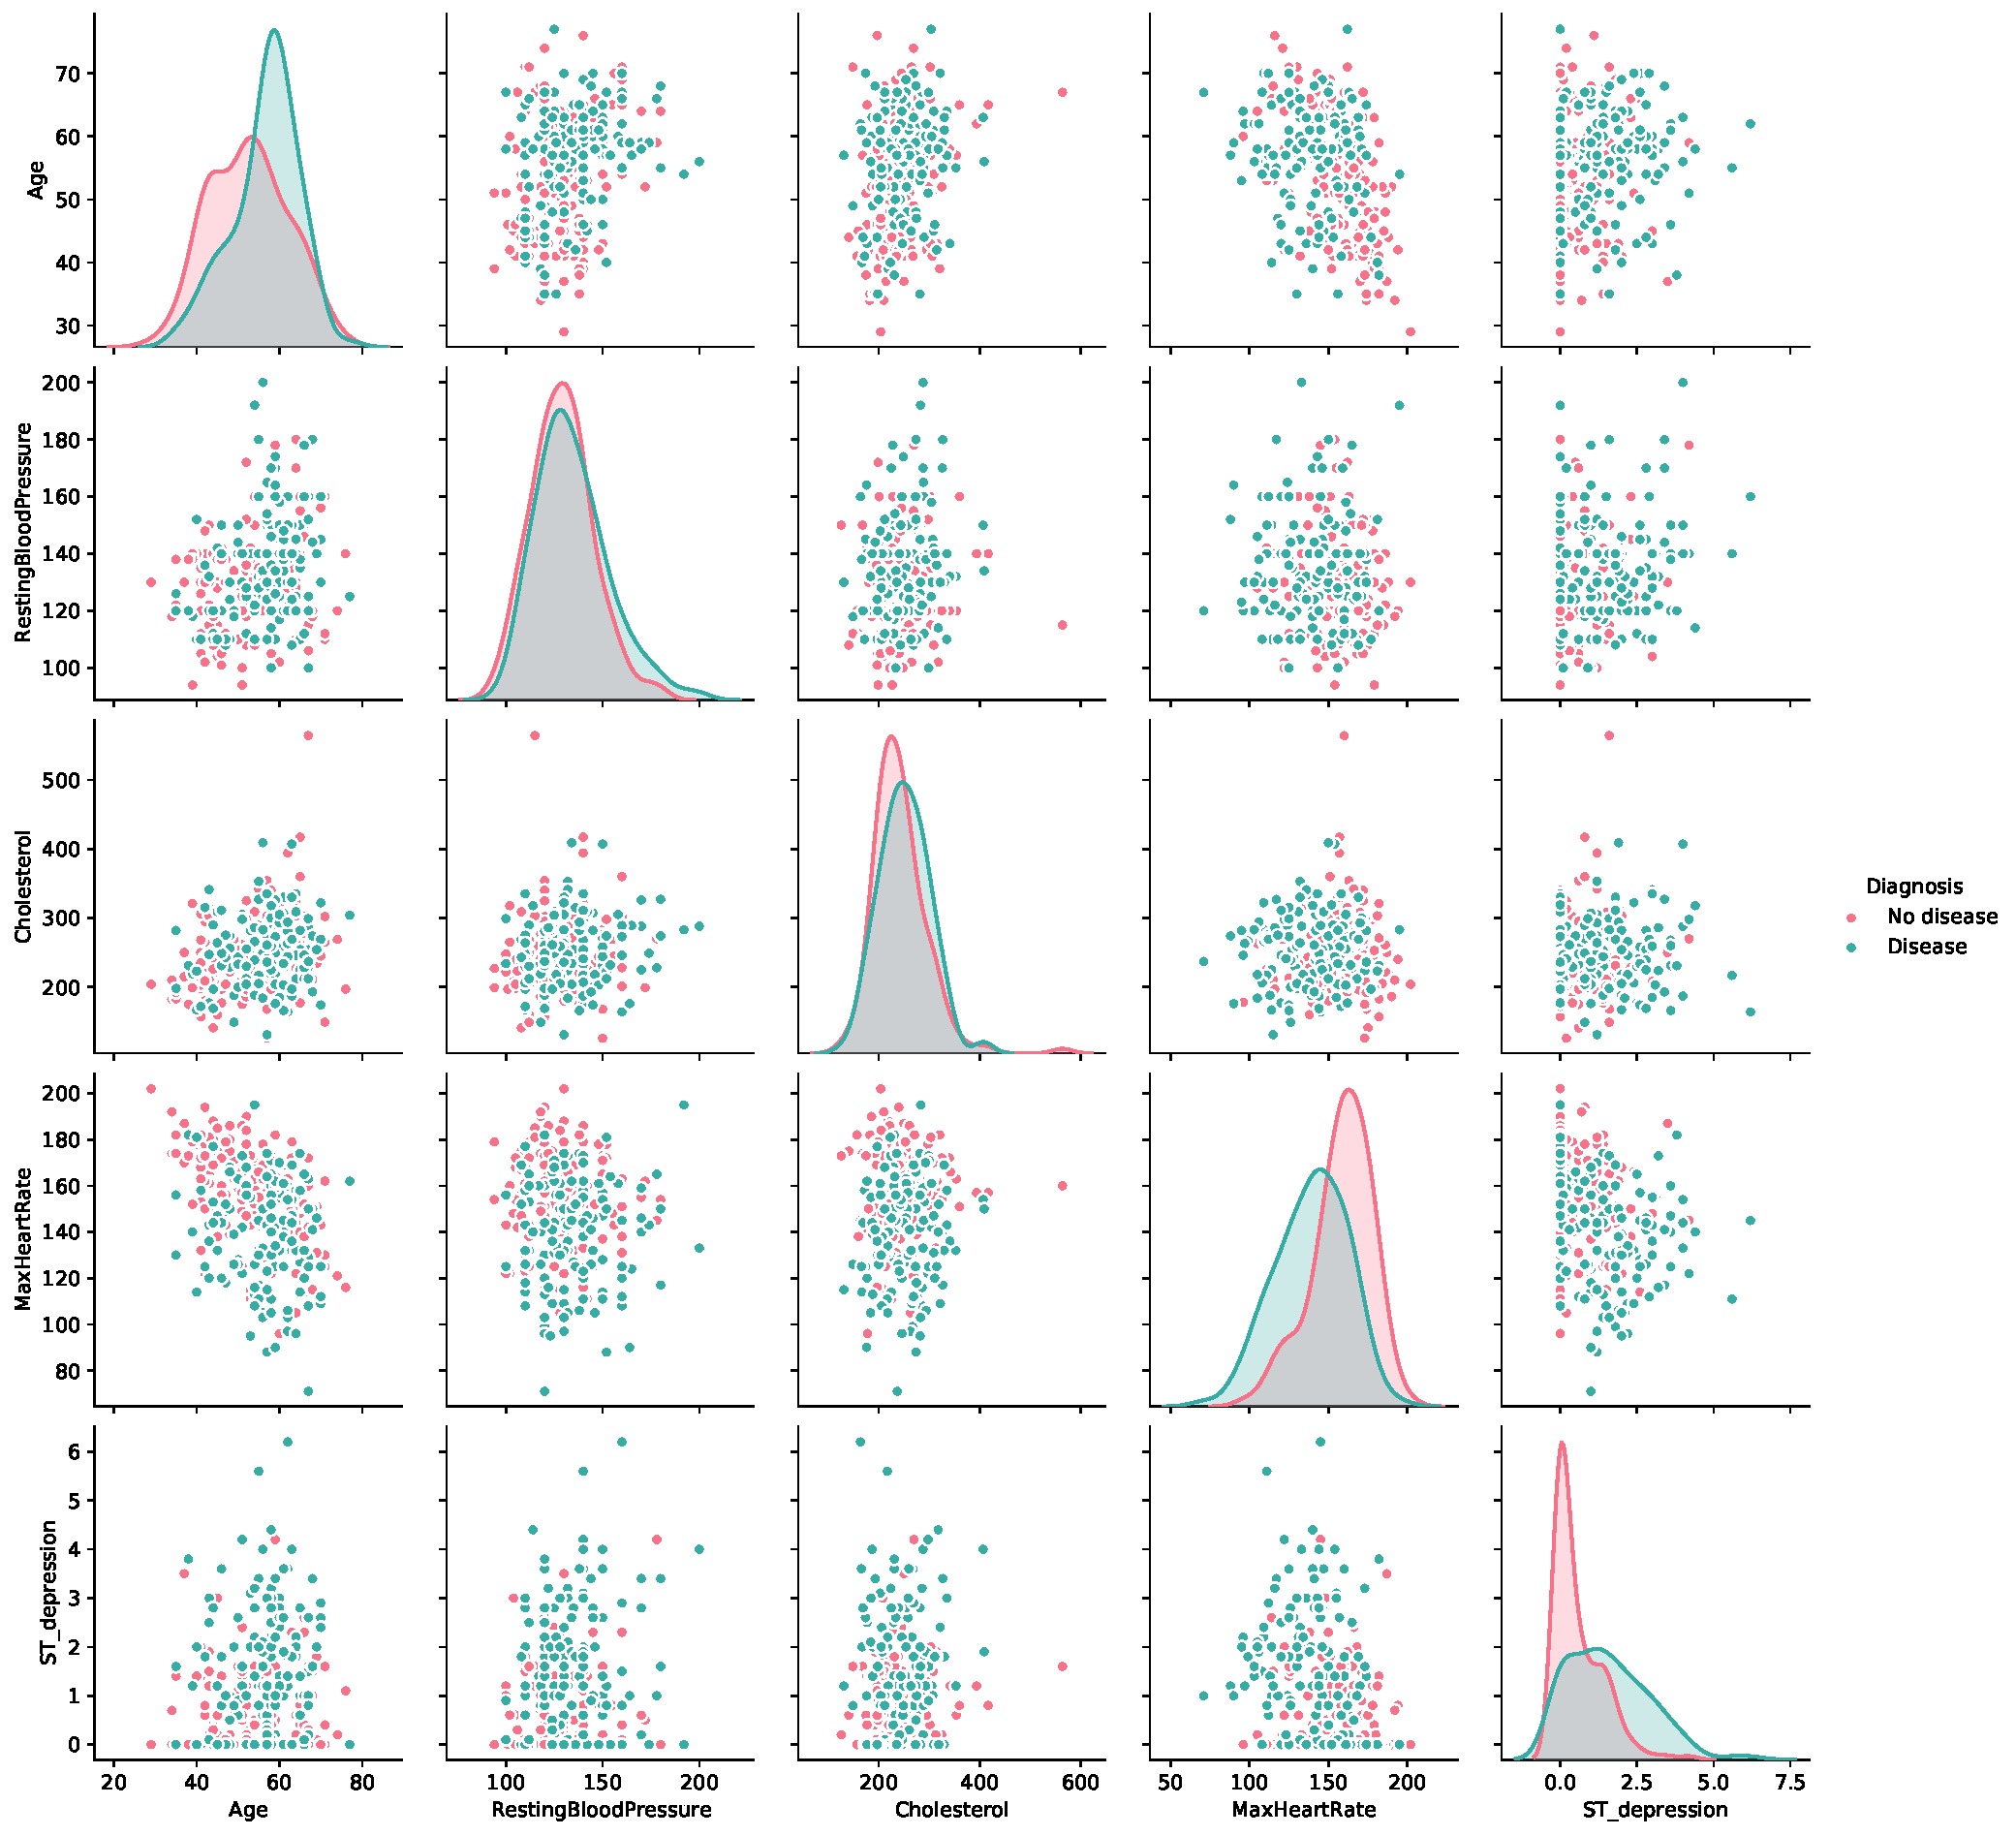
\includegraphics[width=0.8\linewidth]{images/correlation_scatter.pdf}}
    \caption{Scatter plots of the correlation between the features and the diagnosis}
    \label{fig1}
\end{figure}

From the gathered data it can also be concluded that the percentage of patience without heart problems in this sample is 54.13\%.

\begin{figure}[htbp]
    \centerline{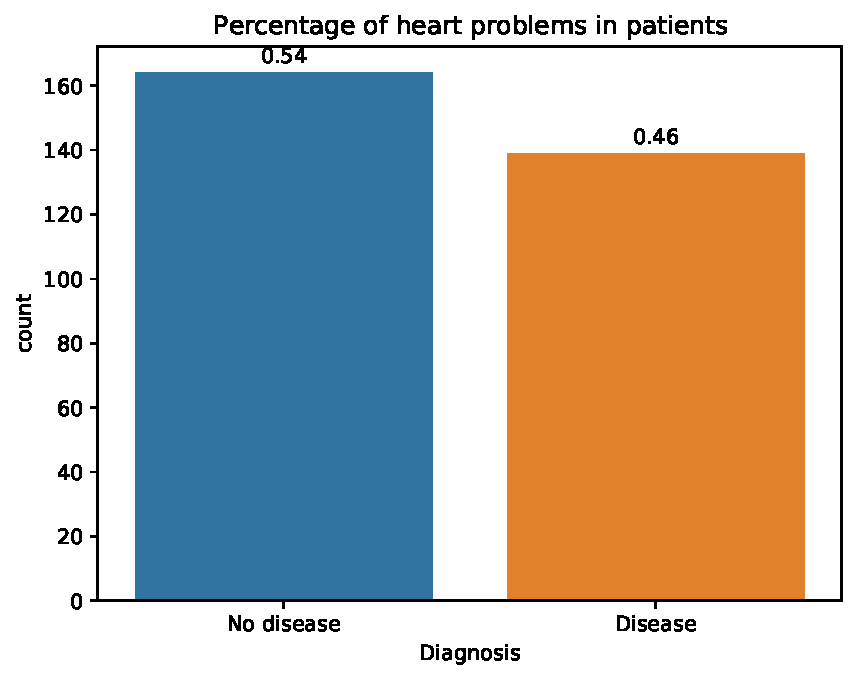
\includegraphics[width=0.7\linewidth]{images/percentage_general.pdf}}
    \caption{Distribution of heart disease in patients}
    \label{fig2}
\end{figure}

\section{Data Preprocessing}

Before training the models the data had to be prepared by filling the missing values on some of the features. This was achieved by giving the mean value for that feature if it was a numeric value or the most common value if it was categorical.\\
The data was then shuffled and split in two sets: one for training and another one for testing and cross-validation with the distribution of 80\% and 20\% respectively.

\section{Model training and tuning}

\subsection{Logistic Regression}

\subsection{Naive Bayes}

\subsection{K Nearest Neighbors}

\subsection{Decision Tree}

\subsection{Random Forest}

\section{Results}

\section{Conclusion}

\begin{thebibliography}{00}
    \bibitem{b1} Hungarian Institute of Cardiology. Budapest: Andras Janosi, M.D.
    \bibitem{b2} University Hospital, Zurich, Switzerland: William Steinbrunn, M.D.
    \bibitem{b3} University Hospital, Basel, Switzerland: Matthias Pfisterer, M.D.
    \bibitem{b4} V.A. Medical Center, Long Beach and Cleveland Clinic Foundation:Robert Detrano, M.D., Ph.D.
    \bibitem{b5} Dua, D. and Graff, C. (2019). UCI Machine Learning Repository [http://archive.ics.uci.edu/ml]. Irvine, CA: University of California, School of Information and Computer Science.
\end{thebibliography}

\end{document}
